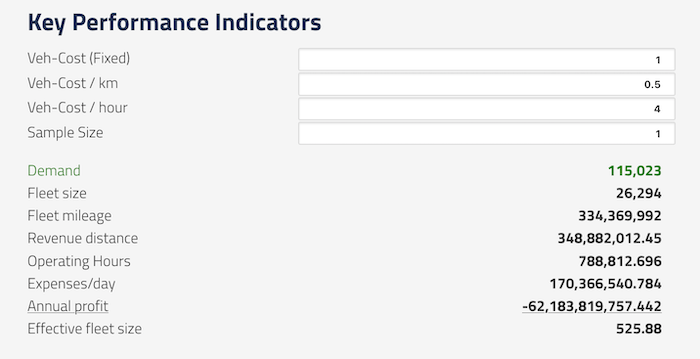
\includegraphics{assets/topsheet.png} \emph{Example ``topsheet''
calculation table}

\hypertarget{introduction}{%
\subsection{Introduction}\label{introduction}}

Calculation tables (formerly called ``topsheets'') are for creating and
displaying a simple table of calculations, based on the CSV and XML data
files in run folders. This can be useful for generating summary
statistics, key performance indicators, etc.

\begin{itemize}
\tightlist
\item
  A calculation table is defined in a YAML file which must be named
  \texttt{table-*.yaml}. (formerly \texttt{topsheet-*}.
\item
  A separate table will be displayed for every topsheet*.yaml file found
  in a run folder.
\end{itemize}

\hypertarget{including-calculation-tables-in-dashboards}{%
\subsection{Including Calculation tables in
dashboards}\label{including-calculation-tables-in-dashboards}}

Use the dashboard \texttt{type:\ table} to include a calculation table
in a dashboard. The table configuration is still stored in a separate
file, and is reference in the \texttt{configFile} parameter. See below:

\begin{Shaded}
\begin{Highlighting}[]
\FunctionTok{layout}\KeywordTok{:}
\AttributeTok{  }\FunctionTok{row1}\KeywordTok{:}
\AttributeTok{    }\KeywordTok{{-}}\AttributeTok{ }\FunctionTok{type}\KeywordTok{:}\AttributeTok{ table}
\AttributeTok{      }\FunctionTok{title}\KeywordTok{:}\AttributeTok{ }\StringTok{"Trips by Time of Day and Purpose"}
\AttributeTok{      }\FunctionTok{description}\KeywordTok{:}\AttributeTok{ }\StringTok{"Hourly summary"}
\AttributeTok{      }\FunctionTok{configFile}\KeywordTok{:}\AttributeTok{ }\StringTok{"topsheet{-}3{-}drt{-}Cost.yml"}
\end{Highlighting}
\end{Shaded}

\hypertarget{project-level-.topsheets-folders}{%
\subsection{Project-level ``.topsheets''
folders}\label{project-level-.topsheets-folders}}

Table definition files can also be saved in a folder named
\texttt{.topsheets} \textbf{anywhere above the current run folder} in
the folder hierarchy.

All topsheets found in the folder tree will be displayed if possible; if
duplicate names are found in higher levels, the topsheet definition
found in the closest level to the current folder will be the one
created.

\hypertarget{example-calculation-table}{%
\subsection{Example calculation table}\label{example-calculation-table}}

\begin{Shaded}
\begin{Highlighting}[]
\CommentTok{\# Topsheet Test}
\FunctionTok{title}\KeywordTok{:}\AttributeTok{ Summary: Key Performance Indicators}

\CommentTok{\# Input files {-}{-}{-}{-}{-}{-}{-}{-}{-}{-}{-}{-}{-}{-}{-}{-}{-}{-}{-}{-}{-}{-}{-}{-}{-}}
\FunctionTok{files}\KeywordTok{:}
\AttributeTok{  }\FunctionTok{customers}\KeywordTok{:}
\AttributeTok{    }\FunctionTok{file}\KeywordTok{:}\AttributeTok{ }\StringTok{"*customer\_stats\_drt.csv"}\CommentTok{    \# note wildcard}
\AttributeTok{    }\FunctionTok{useLastRow}\KeywordTok{:}\AttributeTok{ }\CharTok{true}\CommentTok{                   \# useLastRow: only save the last row of this CSV;}
\CommentTok{                                       \# good for modestats.txt, etc}
\AttributeTok{  }\FunctionTok{personMoneyEvents}\KeywordTok{:}
\AttributeTok{    }\FunctionTok{file}\KeywordTok{:}\AttributeTok{ }\StringTok{"*personMoneyEventsSums.tsv"}\CommentTok{ \# The entire CSV is be saved as an array of}
\CommentTok{                                       \# key:value objects}
\AttributeTok{  }\FunctionTok{drtVehicles}\KeywordTok{:}
\AttributeTok{    }\FunctionTok{file}\KeywordTok{:}\AttributeTok{ }\StringTok{"*drt\_vehicles.xml.gz"}\CommentTok{       \# This is an XML file.}
\AttributeTok{    }\FunctionTok{xmlElements}\KeywordTok{:}\AttributeTok{ }\StringTok{\textquotesingle{}vehicles.vehicle\textquotesingle{}}\CommentTok{    \# Create an array from all \textless{}vehicle\textgreater{} tags which}
\CommentTok{                                       \# are inside the \textless{}vehicles\textgreater{} tag}

\CommentTok{\# USER ENTRIES {-}{-}{-}{-}{-}{-}{-}{-}{-}{-}{-}{-}{-}{-}{-}{-}{-}{-}{-}{-}{-}{-}{-}{-}}
\CommentTok{\# These are text entry boxes in the UI,}
\CommentTok{\# with default values that can be edited by the user}
\FunctionTok{userEntries}\KeywordTok{:}
\AttributeTok{  }\FunctionTok{vehCost\_fix}\KeywordTok{:}
\AttributeTok{    }\FunctionTok{title\_en}\KeywordTok{:}\AttributeTok{ Veh{-}Cost (Fixed)}
\AttributeTok{    }\FunctionTok{title\_de}\KeywordTok{:}\AttributeTok{ Veh{-}Cost (Fixed)}
\AttributeTok{    }\FunctionTok{value}\KeywordTok{:}\AttributeTok{ }\FloatTok{1.0}
\AttributeTok{  }\FunctionTok{vehCost\_km}\KeywordTok{:}
\AttributeTok{    }\FunctionTok{title\_en}\KeywordTok{:}\AttributeTok{ Veh{-}Cost / km}
\AttributeTok{    }\FunctionTok{title\_de}\KeywordTok{:}\AttributeTok{ Veh{-}Cost / km}
\AttributeTok{    }\FunctionTok{value}\KeywordTok{:}\AttributeTok{ }\FloatTok{0.50}
\AttributeTok{  }\FunctionTok{sampleSize}\KeywordTok{:}
\AttributeTok{    }\FunctionTok{title}\KeywordTok{:}\AttributeTok{ }\StringTok{"Sample Size"}
\AttributeTok{    }\FunctionTok{value}\KeywordTok{:}\AttributeTok{ }\FloatTok{0.10}

\CommentTok{\# Calculations {-}{-}{-}{-}{-}{-}{-}{-}{-}{-}{-}{-}{-}{-}{-}{-}{-}{-}{-}{-}{-}{-}{-}{-}{-}{-}{-}{-}{-}{-}{-}{-}{-}{-}{-}{-}{-}{-}{-}{-}{-}{-}{-}{-}}
\CommentTok{\# These are calculated as if in a script, from top to bottom.}
\CommentTok{\# The language is very simple, you generally can only}
\CommentTok{\# do one operation per line. Thus you will probably need}
\CommentTok{\# to calculate a few intermediate variables which can}
\CommentTok{\# be referenced in later lines. Then output the final}
\CommentTok{\# values in the "outputs" section, below.}

\FunctionTok{calculations}\KeywordTok{:}
\CommentTok{  \# Constants first}
\AttributeTok{  }\FunctionTok{userCost\_km}\KeywordTok{:}\AttributeTok{ }\FloatTok{0.25}
\AttributeTok{  }\FunctionTok{userCost\_fix}\KeywordTok{:}\AttributeTok{ }\FloatTok{3.00}
\CommentTok{  \# \{Brackets\} refer to data value substitutions.}

\CommentTok{  \# rides: from the customers data, get the value of the rides column}
\CommentTok{  \# Note the customers file had "useLastRow" set to true, so it will only use the final}
\CommentTok{  \# values found in that CSV}
\AttributeTok{  }\FunctionTok{rides}\KeywordTok{:}\AttributeTok{ }\StringTok{\textquotesingle{}\{customers.rides\}\textquotesingle{}}

\CommentTok{  \# In general, if a calculation inside \{brackets\} refers to an array, the calculation will}
\CommentTok{  \# return the SUM of whatever values that expression refers to.}

\CommentTok{  \# opHours: the drtVehicles file is an array of elements that each have t\_1 and t\_0.}
\CommentTok{  \# This eqn takes the SUM of all t\_1 values, subtracts the SUM of all t\_0 values,}
\CommentTok{  \# and divides this by 3600}
\CommentTok{  \# Arrays can be reduced with @sum, @count, @min, @max, @mean, @first, @last.}
\AttributeTok{  }\FunctionTok{opHours}\KeywordTok{:}\AttributeTok{ }\StringTok{\textquotesingle{}( \{@sum(drtVehicles.t\_1)\} {-} \{@sum(drtVehicles.t\_0)\}) / 3600\textquotesingle{}}

\CommentTok{  \# operatingHours: this takes the value of opHours just calculated and}
\CommentTok{  \# multiplies it by the sampleSize found in the UI entry fields}
\AttributeTok{  }\FunctionTok{operatingHours}\KeywordTok{:}\AttributeTok{ }\StringTok{\textquotesingle{}opHours * sampleSize \^{} ({-}0.662)\textquotesingle{}}

\CommentTok{  \# drtFares: This uses the @filter function to select a subset of the rows in the CSV.}
\CommentTok{  \# drtFares will be an array of rows from personMoneyEvents data where}
\CommentTok{  \# the purpose field equals the string "drtFare"}
\AttributeTok{  }\FunctionTok{drtFares}\KeywordTok{:}\AttributeTok{ }\StringTok{\textquotesingle{}@filter(personMoneyEvents.purpose == drtFare)\textquotesingle{}}

\CommentTok{  \# userFare: drtFares above is an array, so this will be the SUM of the values in the}
\CommentTok{  \# sumAmount column of that filtered dataset.}
\AttributeTok{  }\FunctionTok{userFare}\KeywordTok{:}\AttributeTok{ }\StringTok{\textquotesingle{}\{drtFares.sumAmount\}\textquotesingle{}}

\CommentTok{  \# the round() function does just that.}
\CommentTok{  \# Any functions from the Nerdamer library are valid:}
\CommentTok{  \# https://nerdamer.com/documentation.html}
\AttributeTok{  }\FunctionTok{fleetMileage}\KeywordTok{:}\AttributeTok{ }\StringTok{\textquotesingle{}round(totalDistance * sampleSize \^{} ({-}0.928))\textquotesingle{}}

\AttributeTok{  }\FunctionTok{expensesPerDay}\KeywordTok{:}\AttributeTok{ }\StringTok{\textquotesingle{}fleetSize*vehCost\_fix + fleetMileage*vehCost\_km + operatingHours*vehCost\_hour\textquotesingle{}}
\AttributeTok{  }\FunctionTok{annualProfit}\KeywordTok{:}\AttributeTok{ }\StringTok{\textquotesingle{}365 * (incomePerDay {-} expensesPerDay)\textquotesingle{}}

\CommentTok{\# Table rows {-}{-}{-}{-}{-}{-}{-}{-}{-}{-}{-}{-}{-}{-}{-}{-}{-}{-}{-}{-}{-}{-}{-}{-}{-}{-}{-}}
\CommentTok{\# These values (calculated above) will actually be shown in the table.}
\CommentTok{\# Use "title" if you only need one language, otherwise set title\_en and title\_de}

\CommentTok{\# style can use any CSS property, most likely you will only need}
\CommentTok{\# color, backgroundColor, textDecoration, fontWeight}

\FunctionTok{outputs}\KeywordTok{:}
\AttributeTok{  }\KeywordTok{{-}}\AttributeTok{ }\FunctionTok{title\_en}\KeywordTok{:}\AttributeTok{ Demand}
\AttributeTok{    }\FunctionTok{title\_de}\KeywordTok{:}\AttributeTok{ Nachfrage}
\AttributeTok{    }\FunctionTok{value}\KeywordTok{:}\AttributeTok{ demand}
\AttributeTok{    }\FunctionTok{style}\KeywordTok{:}\AttributeTok{ }\KeywordTok{\{}\AttributeTok{ }\FunctionTok{color}\KeywordTok{:}\AttributeTok{ green}\KeywordTok{\}}

\AttributeTok{  }\KeywordTok{{-}}\AttributeTok{ }\FunctionTok{title}\KeywordTok{:}\AttributeTok{ Fleet size}
\AttributeTok{    }\FunctionTok{value}\KeywordTok{:}\AttributeTok{ fleetSize}

\AttributeTok{  }\KeywordTok{{-}}\AttributeTok{ }\FunctionTok{title\_en}\KeywordTok{:}\AttributeTok{ Annual profit}
\AttributeTok{    }\FunctionTok{title\_de}\KeywordTok{:}\AttributeTok{ Annual profit}
\AttributeTok{    }\FunctionTok{value}\KeywordTok{:}\AttributeTok{ annualProfit}
\AttributeTok{    }\FunctionTok{style}\KeywordTok{:}\AttributeTok{ }\KeywordTok{\{}\AttributeTok{ }\FunctionTok{textDecoration}\KeywordTok{:}\AttributeTok{ underline }\KeywordTok{\}}

\AttributeTok{  }\KeywordTok{{-}}\AttributeTok{ }\FunctionTok{title\_en}\KeywordTok{:}\AttributeTok{ Effective fleet size}
\AttributeTok{    }\FunctionTok{title\_de}\KeywordTok{:}\AttributeTok{ Effective fleet size}
\AttributeTok{    }\FunctionTok{value}\KeywordTok{:}\AttributeTok{ effectiveFleetSize}
\end{Highlighting}
\end{Shaded}

\hypertarget{detailed-usage-guide}{%
\subsection{Detailed usage guide}\label{detailed-usage-guide}}

A topsheet config is specified in YAML and each top-level section has a
specific purpose.

\textbf{title:} The title of the summary table. You can use
\texttt{title} or a combination of \texttt{title\_en} and
\texttt{title\_de}.

\textbf{files:} Each key in this section will be the name of a dataset
that can be accessed in the calculations below.

\begin{itemize}
\tightlist
\item
  Specify the \texttt{file} name pattern, which can include an asterisk
  to select a pattern if necessary. The \emph{first file that matches
  the pattern} will be used.
\item
  \texttt{useLastRow} can be used to drop all rows except the final row.
  This is useful for some standard MATSim output files such as
  \texttt{modestats.txt} if you only care about the values in the final
  iteration.
\end{itemize}

\textbf{userEntries:} Each key in this section is the name of a field
that will appear at the top of the table, with a default value. The
value of that field can then be used in the calculations below.

\begin{itemize}
\tightlist
\item
  \texttt{title} or \texttt{title\_en} and \texttt{title\_de} will be
  the label for the input entry.
\item
  \texttt{value} is the default value, pre-filled in the form
\end{itemize}

\textbf{calculations:} is a top-down list of calculations that will be
performed in the order they appear. You can perform calculations on the
values in the files and input entries above. This language is not very
sophisticated so you will probably need to create multiple intermediate
calculations if you need something complex. See below for more details
on the calculation engine.

If you cannot specify your calculation using this language, perhaps you
need to run your own post-processing script to generate a simple CSV
with the values you need. And then read that CSV file in, instead!

\textbf{outputs:} each element of this list will be an output row in the
UI table.

\begin{itemize}
\tightlist
\item
  \texttt{value} should be the name of one of the calculated values,
  above. No calculations can be done here!
\item
  \texttt{title} or both \texttt{title\_en} and \texttt{title\_de} will
  be the label for this value
\item
  \texttt{style} can optionally include CSS styling properties, if you
  would like this row to be bold, green, etc. You can use any CSS valid
  styling properties in camelCase format, including typical values such
  as:

  \begin{itemize}
  \tightlist
  \item
    \texttt{color:\ red} for text color. Color names and \#hexcodes are
    valid
  \item
    \texttt{backgroundColor:\ yellow} for highlighting the background
    color of the entire row
  \item
    \texttt{fontWeight:\ bold} for bold text
  \item
    \texttt{textAlign:\ right} for left, right, center aligned values
  \item
    \texttt{textDecoration:\ underline} for underlining
  \item
    Feel free to experiment with other CSS styling!
  \end{itemize}
\end{itemize}

\hypertarget{the-calculation-engine}{%
\subsubsection{The calculation engine}\label{the-calculation-engine}}

Calculations are based on the \href{https://nerdamer.com/}{Nerdamer
javascript calculation engine}, which is pretty advanced but doesn't
know anything about our datasets, so we built a simple
substitute/replace language which grabs values from the data files
before sending the equations to the Nerdamer engine for evaluation.

Every line takes the form:

\begin{verbatim}
variableName: 'equation + with + variables + etc'
\end{verbatim}

where equation components can be constants, values retrieved from the UI
form, variables already calculated, or lookups from the loaded data
files. Typical math and logic operators such as \texttt{+,-,*,/,\^{}}
are all supported.

\textbf{Constants:} are simple, you define the name and the value.

\texttt{sampleRate:\ 0.25}

\textbf{UI Entry Fields:} you can refer to values entered in any UI
fields directly by name.

\texttt{ridership:\ \textquotesingle{}sampleRate\ *\ totalRiders\textquotesingle{}}

\textbf{Filtering datasets:} You can filter a dataset and save that
selection as a new variable name using \textbf{@filter()}. Useful if you
are only interested in a subset of rows.

\texttt{selectedRows:\ @filter(filename.column\ ==\ value)}

will return an array of rows for which the value in the specified file's
column matches the logical expression.

\begin{itemize}
\tightlist
\item
  The test value must always be a numeric or string constant. Do not use
  quotes around strings!
\item
  Valid comparisons are
  \texttt{==\ !=\ \textgreater{}=\ \textless{}=\ \textless{}\ \textgreater{}}
\item
  You cannot filter on multiple comparisons: no ANDs and no ORs. Sorry
\item
  The output is stored as a new array with the name you specify, and can
  then be referenced in later calculations
\end{itemize}

\textbf{Data lookups:} Any elements enclosed in \{curly brackets\} will
trigger a lookup from the loaded data files.

\texttt{myVar:\ \{file.field\}}

sets myVar to the value of the referenced \textbf{file} for the
specified \textbf{field}.

\begin{itemize}
\tightlist
\item
  If \texttt{file} is just one row of data, such as from
  \texttt{useLastRow}, the value of the \texttt{field} column or
  property will be directly used.
\end{itemize}

\textbf{Arrays} can be reduced using several obvious functions:
\textbf{@sum}, \textbf{@count}, \textbf{@min}, \textbf{@max},
\textbf{@mean}, \textbf{@first}, \textbf{@last}. If an array is found in
an equation without one of these functions, the SUM of all values will
be taken by default.

See the example above for more hints on how this works.

\textbf{Special functions: rounding, counting, etc}

Any of the math functions in the
\href{https://nerdamer.com/documentation.html}{Nerdamer documentation}
can theoretically be used, even trigonometry if you like! But more
typically, round(), floor(), int(), etc.
